\section{Задание 5. Аппроксимация RBF-сетью}

\subsection{Постановка задачи}

Используя данные варианта 11 (см. таблицу~\ref{tab:data}), выполнить аппроксимацию функции RBF-сетью (Стратегия 2: градиентный спуск по всем параметрам). Требуется: построить кривую обучения, вычислить невязки, построить модельную поверхность и линии уровня, записать аналитический вид.

\subsection{Математическая модель}

RBF-сеть с $M = 2$ нейронами:

\begin{equation}\label{eq:rbf}
    z(\mathbf{x}) = b + \sum_{j=1}^{M} w_j \cdot \exp\left(-\frac{\|\mathbf{x} - \mathbf{c}_j\|^2}{2\sigma_j^2}\right),
\end{equation}
где $\mathbf{c}_j = (c_{j1}, c_{j2})$ --- центры; $\sigma_j$ --- ширины; $w_j$ --- веса; $b$ --- смещение.

Функция потерь: $L = \frac{1}{N}\sum_{i=1}^{N}(z(\mathbf{x}_i) - z_i)^2$.

\subsection{Алгоритм обучения}

\textbf{Этап 1: Инициализация.}
\begin{itemize}
    \item Центры $\mathbf{c}_j$ определяются методом K-средних (начальные центры --- точки 0 и 2). Результат: $\mathbf{c}_1 = (1.34, 1.66)$, $\mathbf{c}_2 = (3.90, 3.99)$.
    \item Ширины: $\sigma_1 = \sigma_2 = 0.5 \cdot \|\mathbf{c}_1 - \mathbf{c}_2\| = 1.7319$.
    \item Веса $w_j \sim \mathcal{N}(0, 0.5^2)$, $b = 0$.
\end{itemize}

\textbf{Этап 2: Градиентный спуск} с $\eta = 0.1$, 500 эпох. Градиенты:

\begin{align}
    \frac{\partial L}{\partial w_j} &= \frac{2}{N}\sum_{i=1}^{N} e_i \cdot \phi_j(\mathbf{x}_i), \\
    \frac{\partial L}{\partial b} &= \frac{2}{N}\sum_{i=1}^{N} e_i, \\
    \frac{\partial L}{\partial \sigma_j} &= \frac{2}{N}\sum_{i=1}^{N} e_i w_j \phi_j(\mathbf{x}_i) \frac{\|\mathbf{x}_i - \mathbf{c}_j\|^2}{\sigma_j^3}, \\
    \frac{\partial L}{\partial \mathbf{c}_j} &= \frac{2}{N}\sum_{i=1}^{N} e_i w_j \phi_j(\mathbf{x}_i) \frac{\mathbf{x}_i - \mathbf{c}_j}{\sigma_j^2},
\end{align}
где $e_i = z(\mathbf{x}_i) - z_i$, $\phi_j(\mathbf{x}) = \exp\bigl(-\|\mathbf{x} - \mathbf{c}_j\|^2 / (2\sigma_j^2)\bigr)$.

\subsection{Кривая обучения}

\begin{figure}[H]
    \centering
    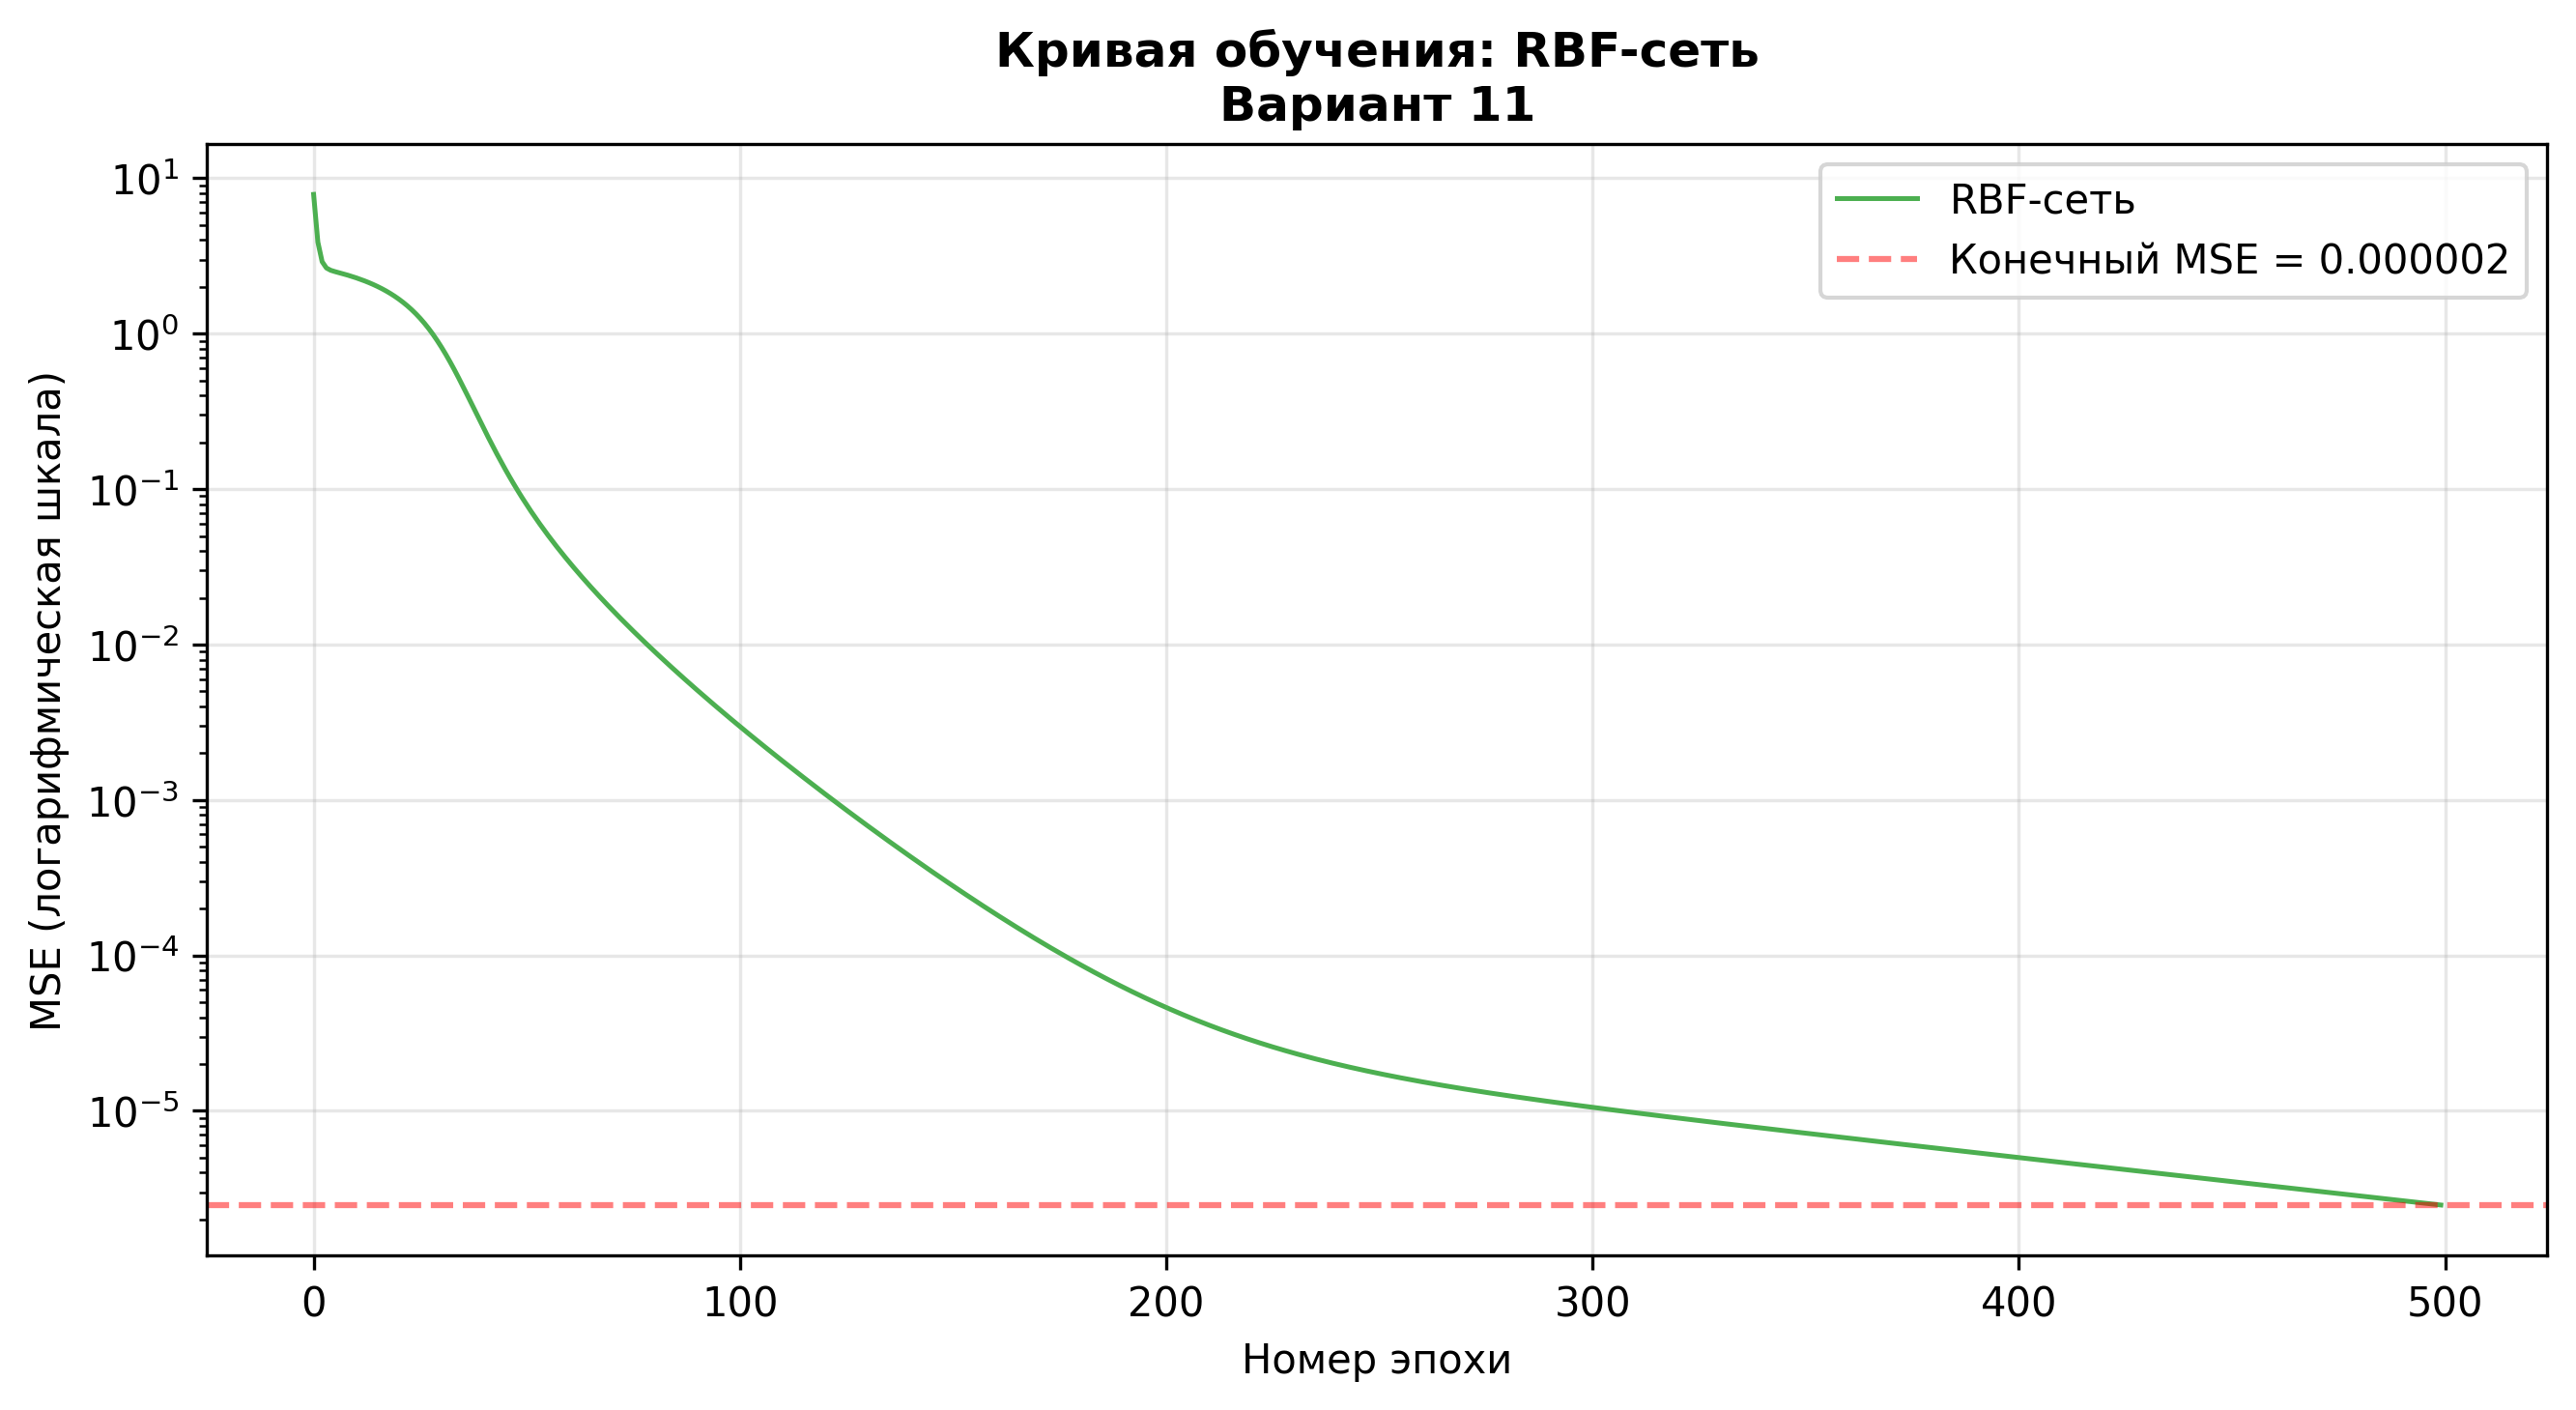
\includegraphics[width=0.85\textwidth]{pic/rbf_learning_curve.png}
    \caption{Кривая обучения RBF-сети (Вариант 11)}
    \label{fig:rbf_learning}
\end{figure}

Начальный MSE = 7.877, конечный --- $2.5 \times 10^{-6}$. Обучение сходится быстро: после $\sim 50$ эпох MSE опускается ниже 1.0, после 300 эпох стабилизируется.

\subsection{Результаты}

\begin{table}[H]
    \centering
    \caption{Оптимальные параметры RBF-сети}
    \label{tab:rbf_params}
    \begin{tabular}{|c|c|c|c|c|}
        \hline
        \textbf{Нейрон} & \textbf{Вес $w_j$} & \textbf{Центр $c_{j1}$} & \textbf{Центр $c_{j2}$} & \textbf{Ширина $\sigma_j$} \\
        \hline
        1 & 2.7715 & 2.5082 & 2.7985 & 1.1862 \\
        2 & 2.2831 & 2.7098 & 2.9521 & 1.2339 \\
        \hline
        \multicolumn{5}{|c|}{Смещение $b = 0.1058$} \\
        \hline
    \end{tabular}
\end{table}

\subsection{Аналитический вид модели}

\begin{equation}\label{eq:rbf_result}
    \begin{aligned}
        z(x,y) = 0.1058 &+ 2.7715 \cdot \exp\left(-\frac{(x - 2.5082)^2 + (y - 2.7985)^2}{2 \cdot 1.1862^2}\right) \\
                         &+ 2.2831 \cdot \exp\left(-\frac{(x - 2.7098)^2 + (y - 2.9521)^2}{2 \cdot 1.2339^2}\right).
    \end{aligned}
\end{equation}

В отличие от варианта 7 (где один нейрон имел вес $\approx 0$), здесь оба нейрона имеют сопоставимые веса (2.77 и 2.28). Это означает, что RBF-сеть использует оба нейрона для моделирования пика, что даёт более гибкую форму по сравнению с одной гауссианой.

\subsection{Таблица невязок}

\begin{table}[H]
    \centering
    \caption{Невязки RBF-сети}
    \label{tab:rbf_residuals}
    \begin{tabular}{|c|c|c|c|c|c|}
        \hline
        \textbf{Точка} & \textbf{$x$} & \textbf{$y$} & \textbf{$z_{факт}$} & \textbf{$z_{модель}$} & \textbf{Невязка} & \textbf{Кв. невязки} \\
        \hline
        0 & 0.85 & 1.12 & 0.73 & 0.7327 & $2.7 \times 10^{-3}$ & $7.0 \times 10^{-6}$ \\
        1 & 1.83 & 2.20 & 3.65 & 3.6486 & $-1.4 \times 10^{-3}$ & $2.0 \times 10^{-6}$ \\
        2 & 2.91 & 3.12 & 4.86 & 4.8609 & $8.8 \times 10^{-4}$ & $7.7 \times 10^{-7}$ \\
        3 & 3.93 & 3.92 & 2.00 & 1.9994 & $-5.9 \times 10^{-4}$ & $3.5 \times 10^{-7}$ \\
        4 & 4.86 & 4.94 & 0.32 & 0.3185 & $-1.5 \times 10^{-3}$ & $2.1 \times 10^{-6}$ \\
        \hline
    \end{tabular}
\end{table}

$\text{MSE} = 2.46 \times 10^{-6}$, $\text{RMSE} = 1.57 \times 10^{-3}$. Невязки малы, модель хорошо описывает данные.

\subsection{Визуализация}

\begin{figure}[H]
    \centering
    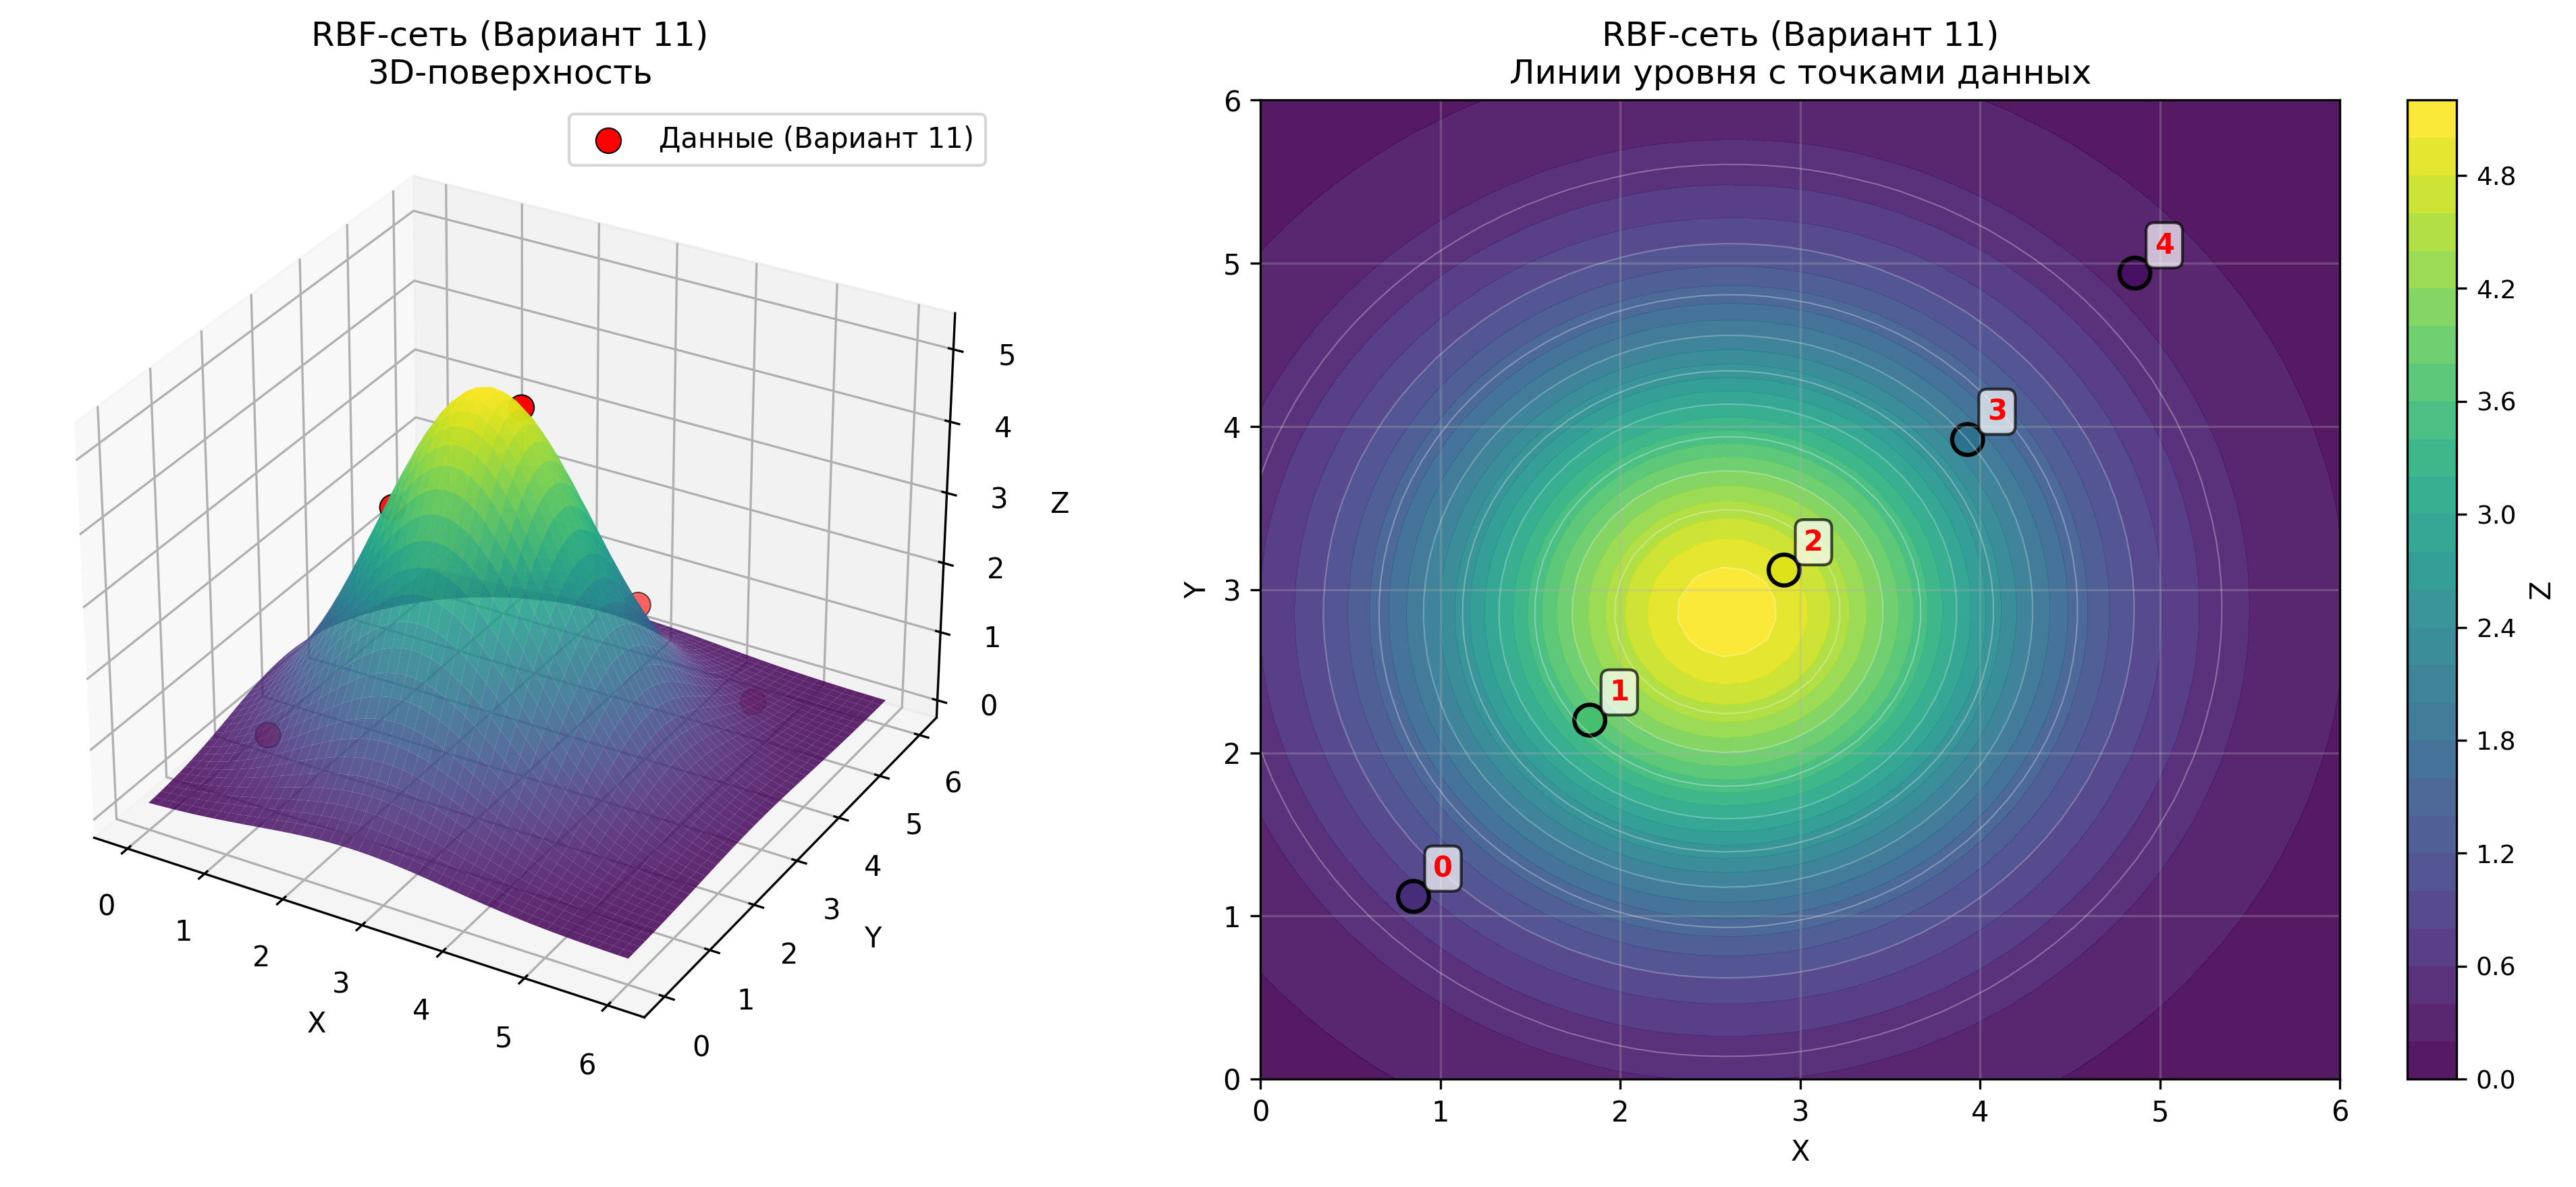
\includegraphics[width=\textwidth]{pic/rbf_model.png}
    \caption{RBF-сеть (Вариант 11): 3D-поверхность (слева) и линии уровня (справа)}
    \label{fig:rbf_model}
\end{figure}

\subsection{Сравнительный анализ}

\begin{table}[H]
    \centering
    \caption{Сводная таблица предсказаний}
    \label{tab:comparison}
    \begin{tabular}{|c|c|c|c|c|c|c|}
        \hline
        \textbf{Точка} & \textbf{$z_{факт}$} & \textbf{Гаус.} & \textbf{Параб.} & \textbf{Const\textsubscript{MSE}} & \textbf{Const\textsubscript{MAE}} & \textbf{RBF} \\
        \hline
        0 & 0.73 & 0.7300 & 0.5967 & 2.3120 & 2.0000 & 0.7327 \\
        1 & 3.65 & 3.6500 & 4.0223 & 2.3120 & 2.0000 & 3.6486 \\
        2 & 4.86 & 4.8600 & 4.5122 & 2.3120 & 2.0000 & 4.8609 \\
        3 & 2.00 & 2.0000 & 2.1919 & 2.3120 & 2.0000 & 1.9994 \\
        4 & 0.32 & 0.3200 & 0.2722 & 2.3120 & 2.0000 & 0.3185 \\
        \hline
    \end{tabular}
\end{table}

\begin{table}[H]
    \centering
    \caption{Сравнение MSE и RMSE}
    \label{tab:mse_comparison}
    \begin{tabular}{|l|c|c|c|}
        \hline
        \textbf{Метод} & \textbf{Парам.} & \textbf{MSE} & \textbf{RMSE} \\
        \hline
        Гауссиана & 7 & $1.0 \times 10^{-10}$ & $8.2 \times 10^{-6}$ \\
        Параболоид & 6 & 0.0633 & 0.2516 \\
        Конст. MSE & 1 & 2.9701 & 1.7234 \\
        Конст. MAE & 1 & 3.0675 & 1.7514 \\
        RBF-сеть & 9 & $2.46 \times 10^{-6}$ & $1.57 \times 10^{-3}$ \\
        \hline
    \end{tabular}
\end{table}

\begin{figure}[H]
    \centering
    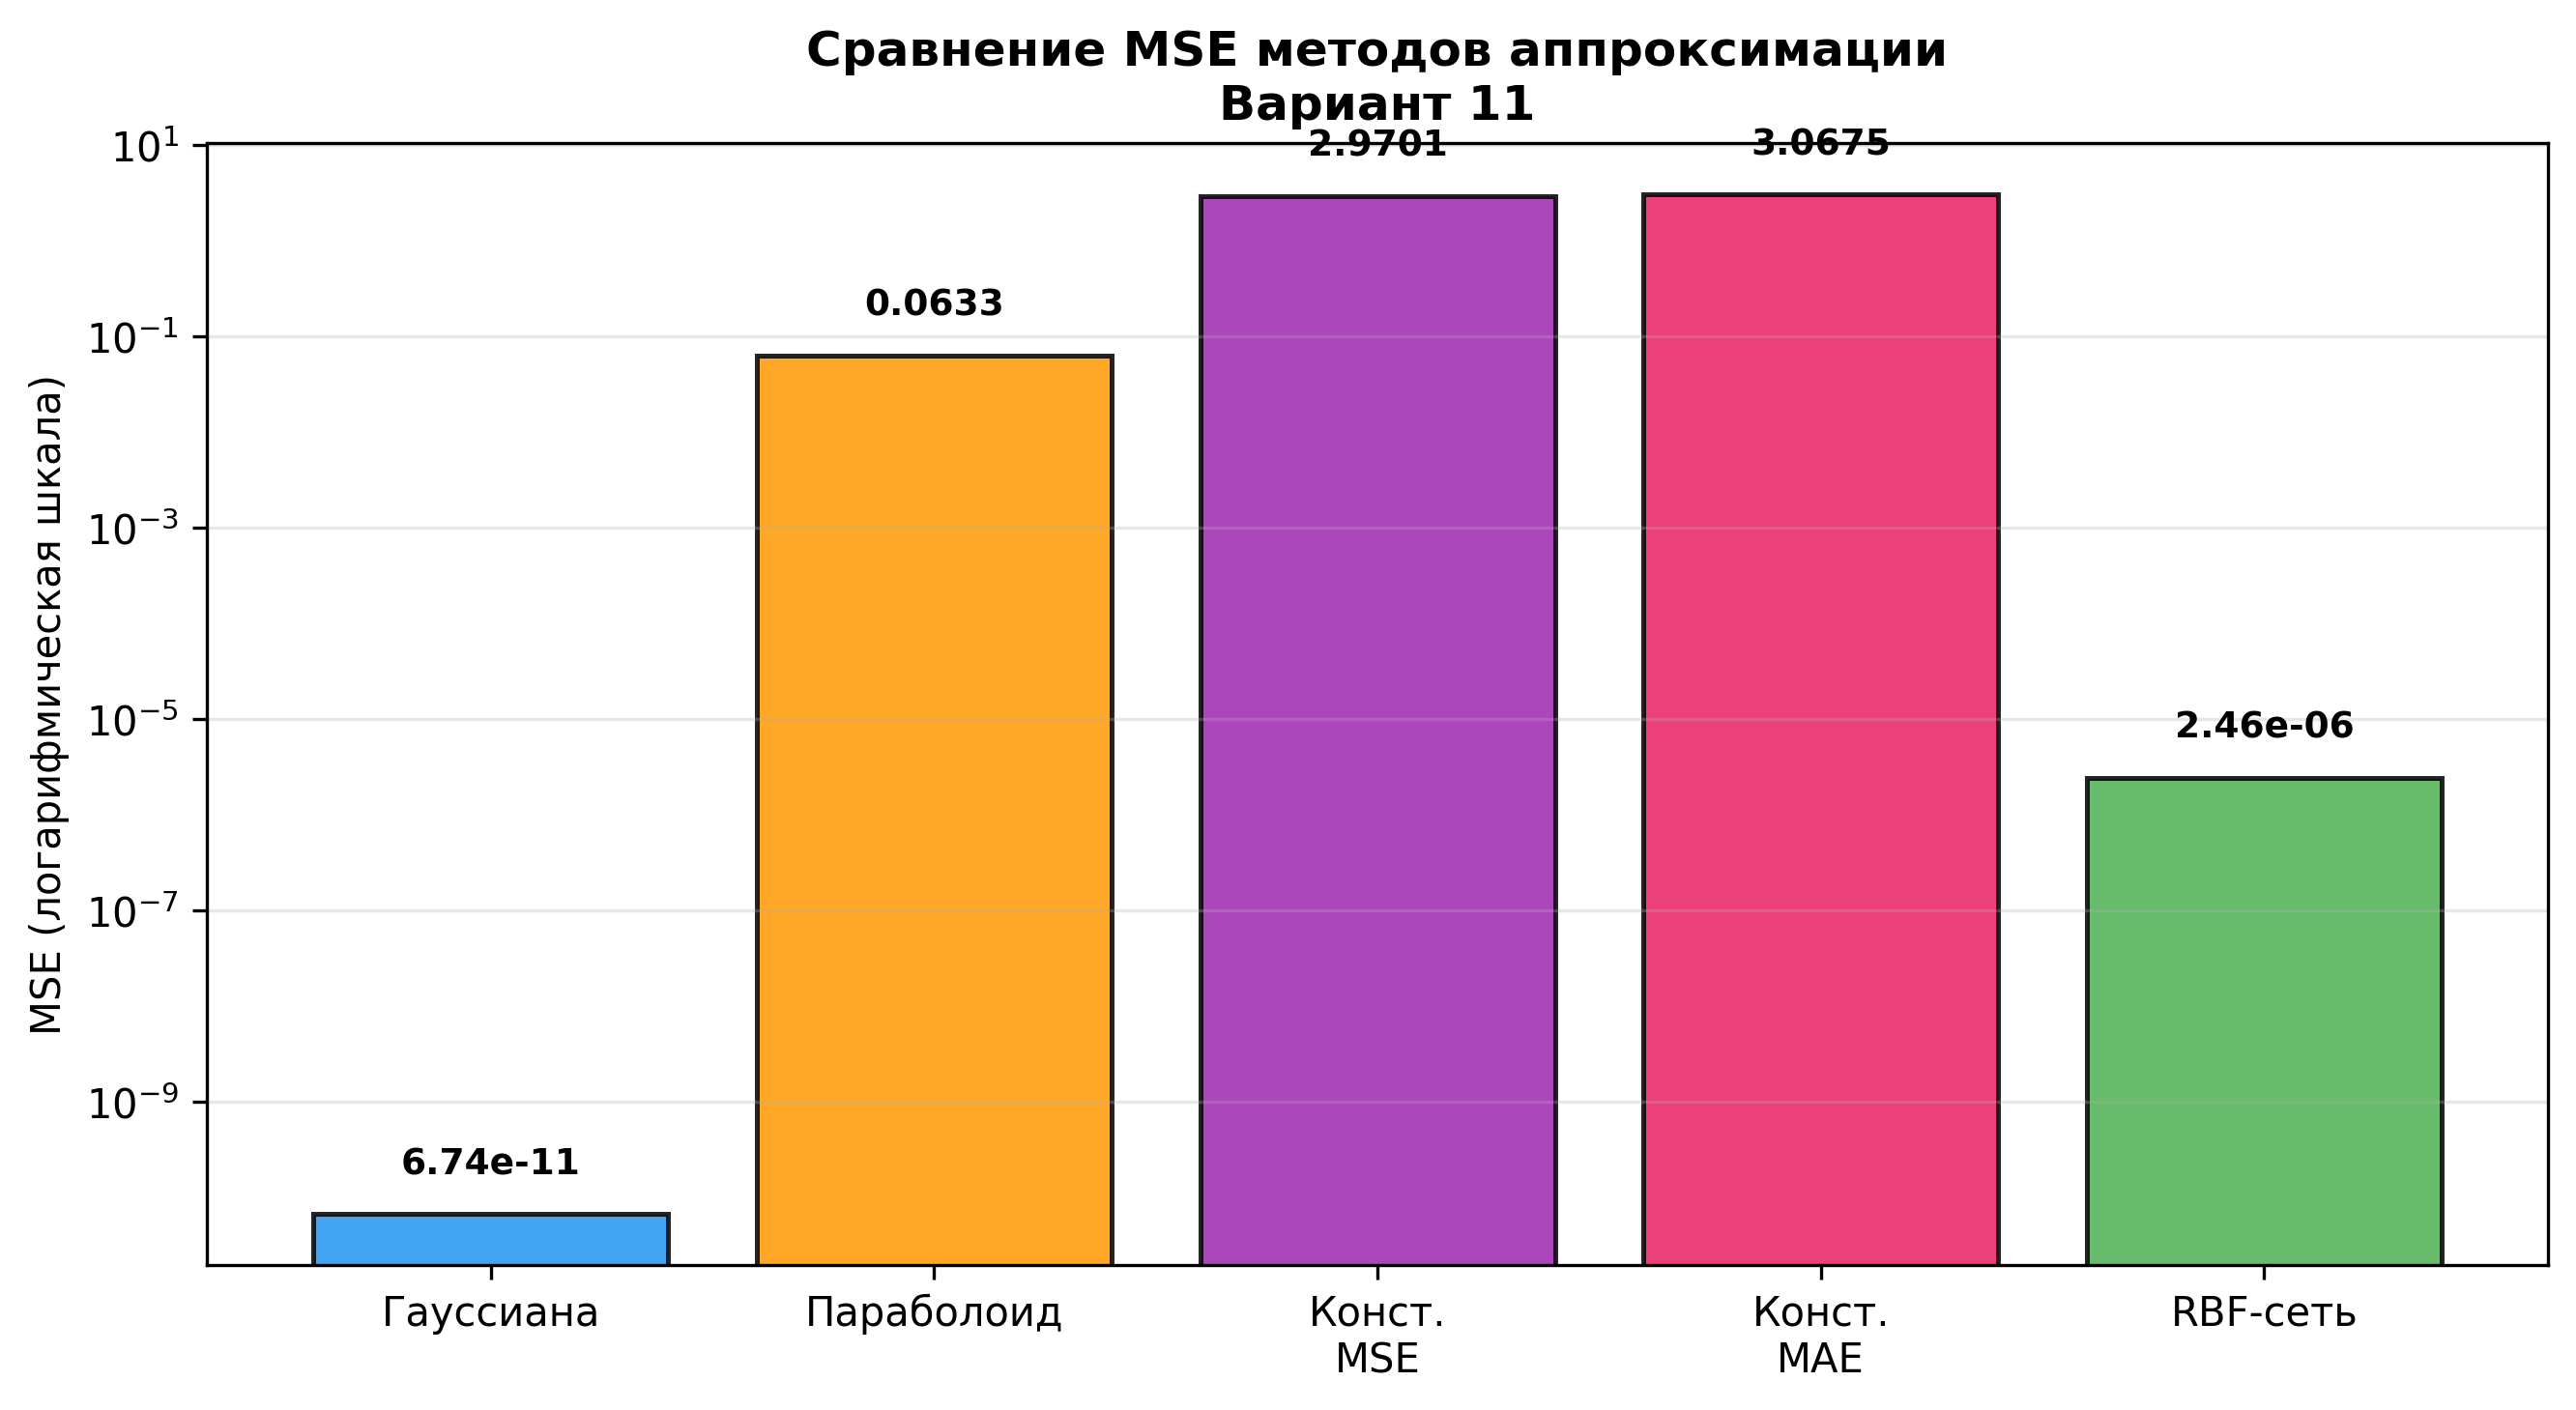
\includegraphics[width=0.8\textwidth]{pic/mse_comparison.png}
    \caption{Сравнение MSE всех методов (Вариант 11)}
    \label{fig:mse_comp}
\end{figure}

\begin{figure}[H]
    \centering
    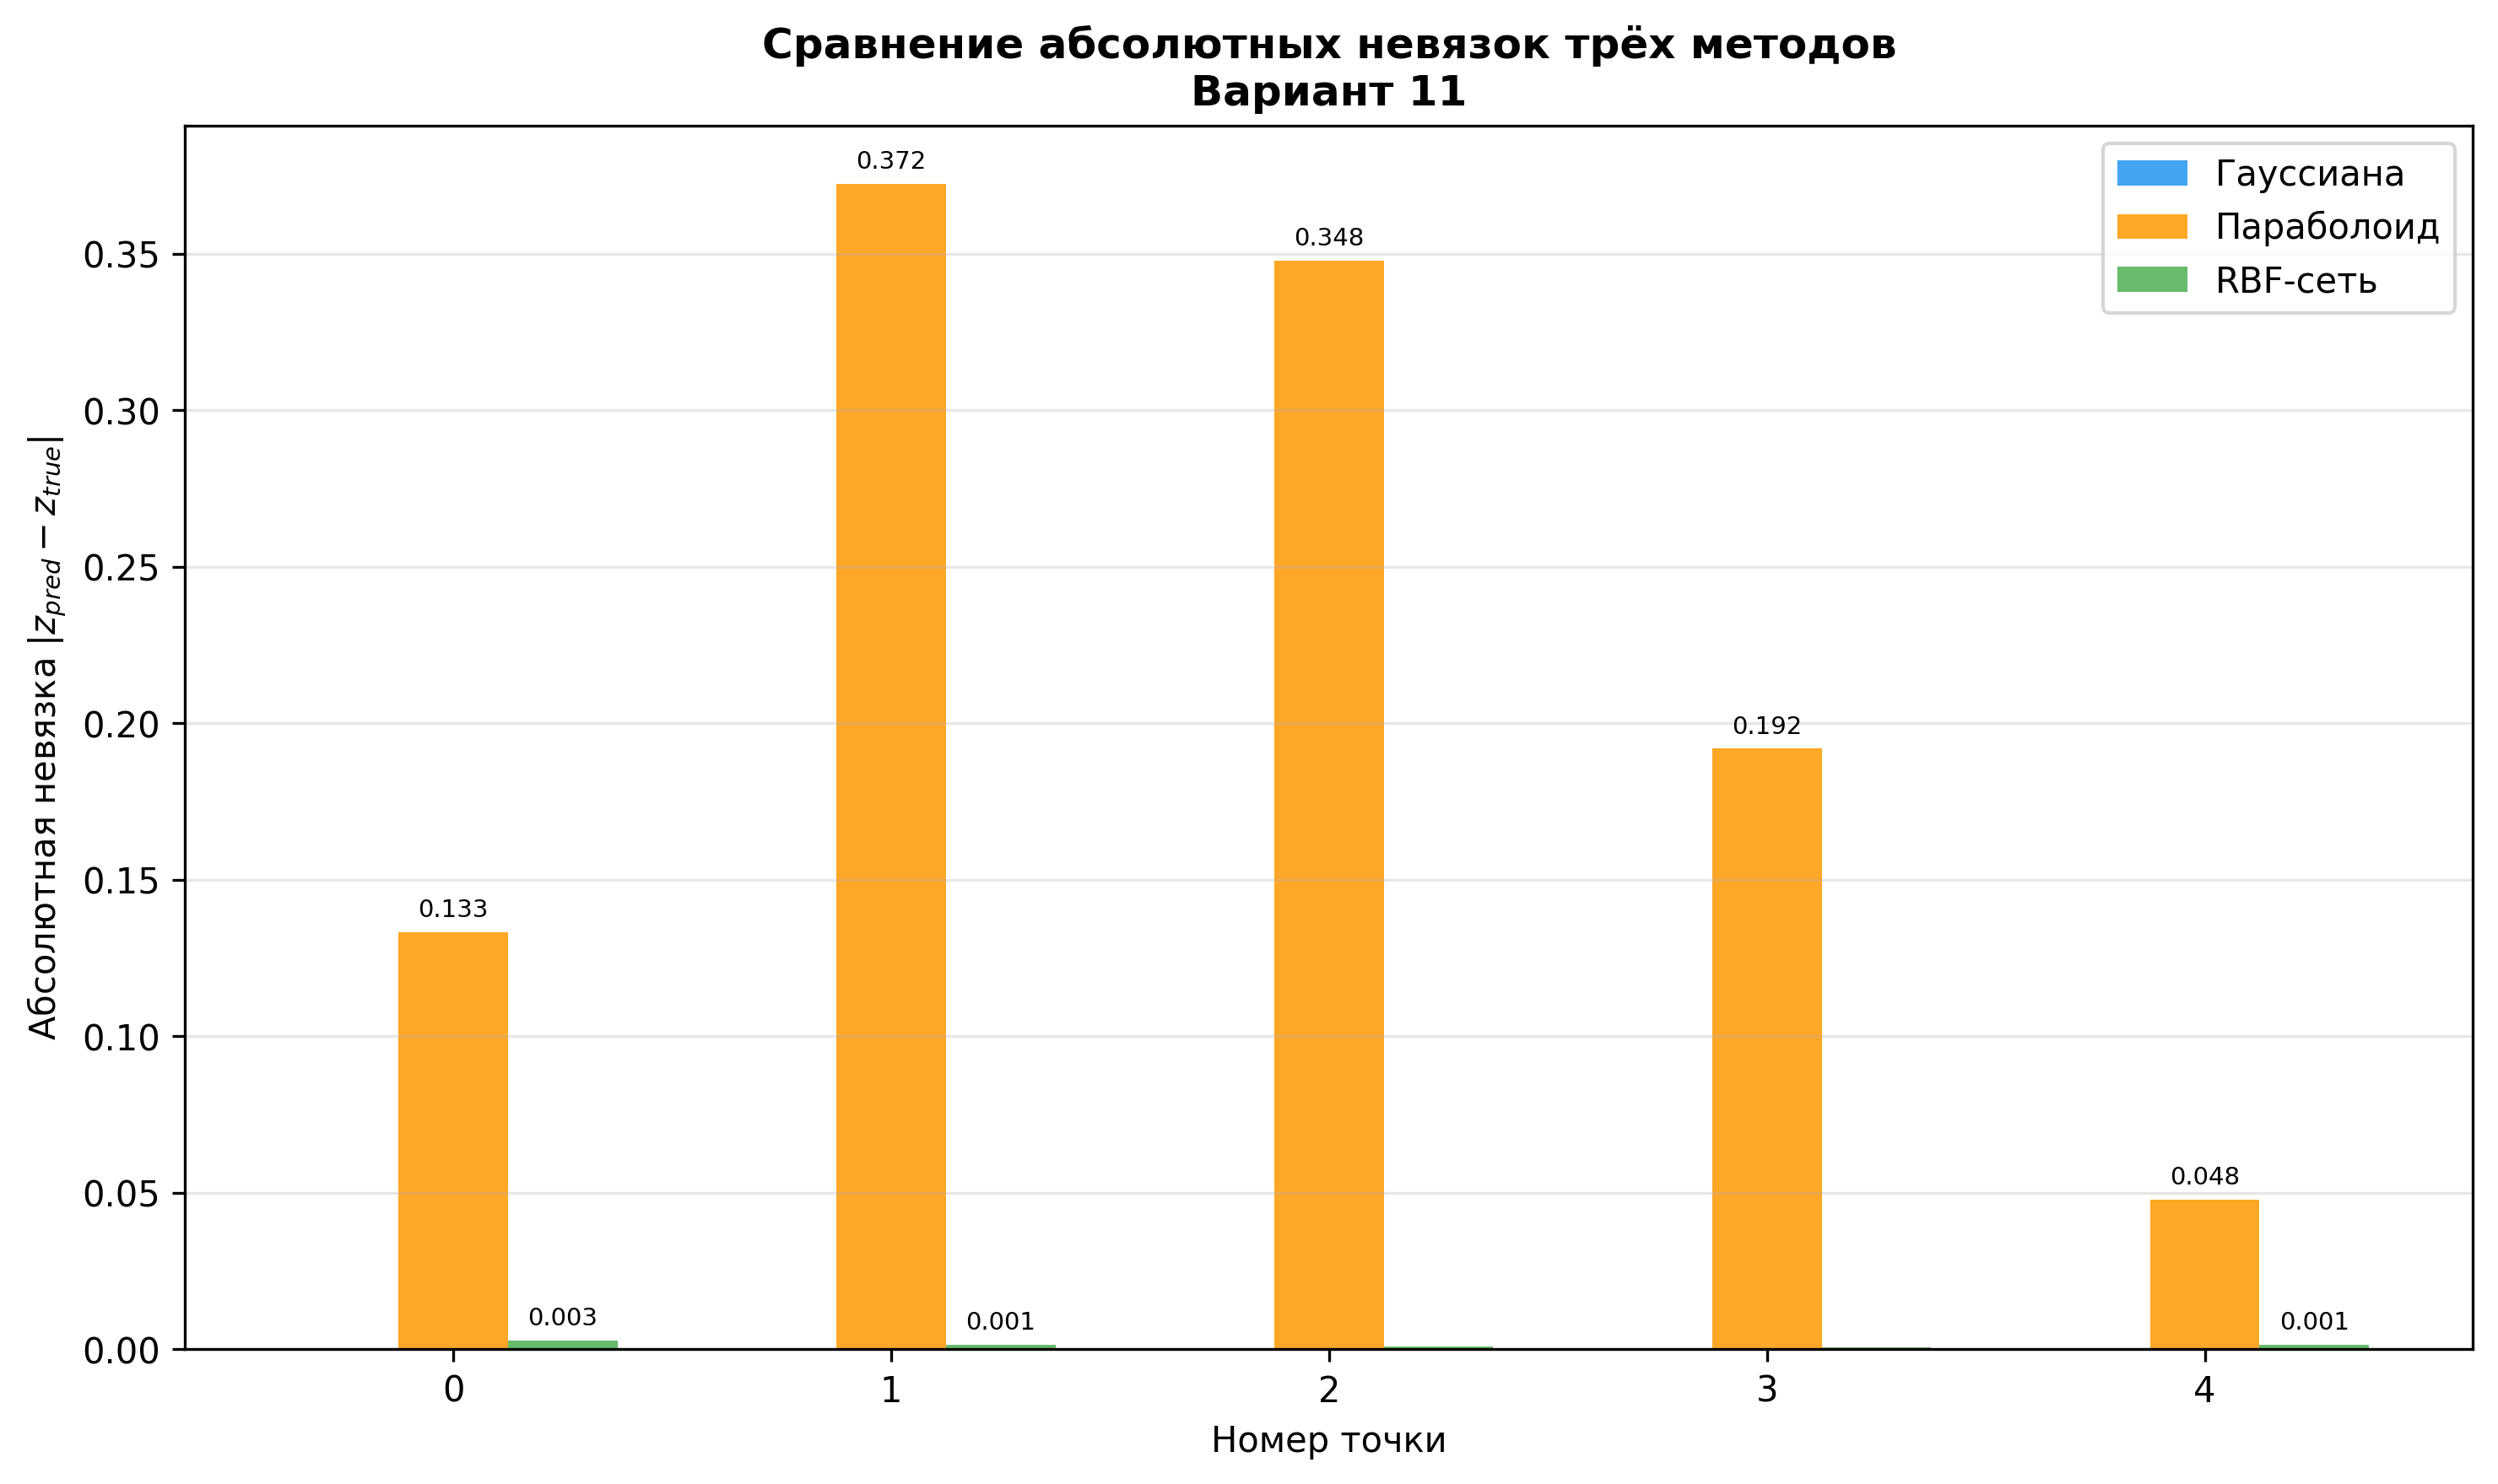
\includegraphics[width=0.85\textwidth]{pic/error_comparison.png}
    \caption{Абсолютные невязки Гауссианы, Параболоида и RBF-сети (Вариант 11)}
    \label{fig:error_comp}
\end{figure}

\begin{figure}[H]
    \centering
    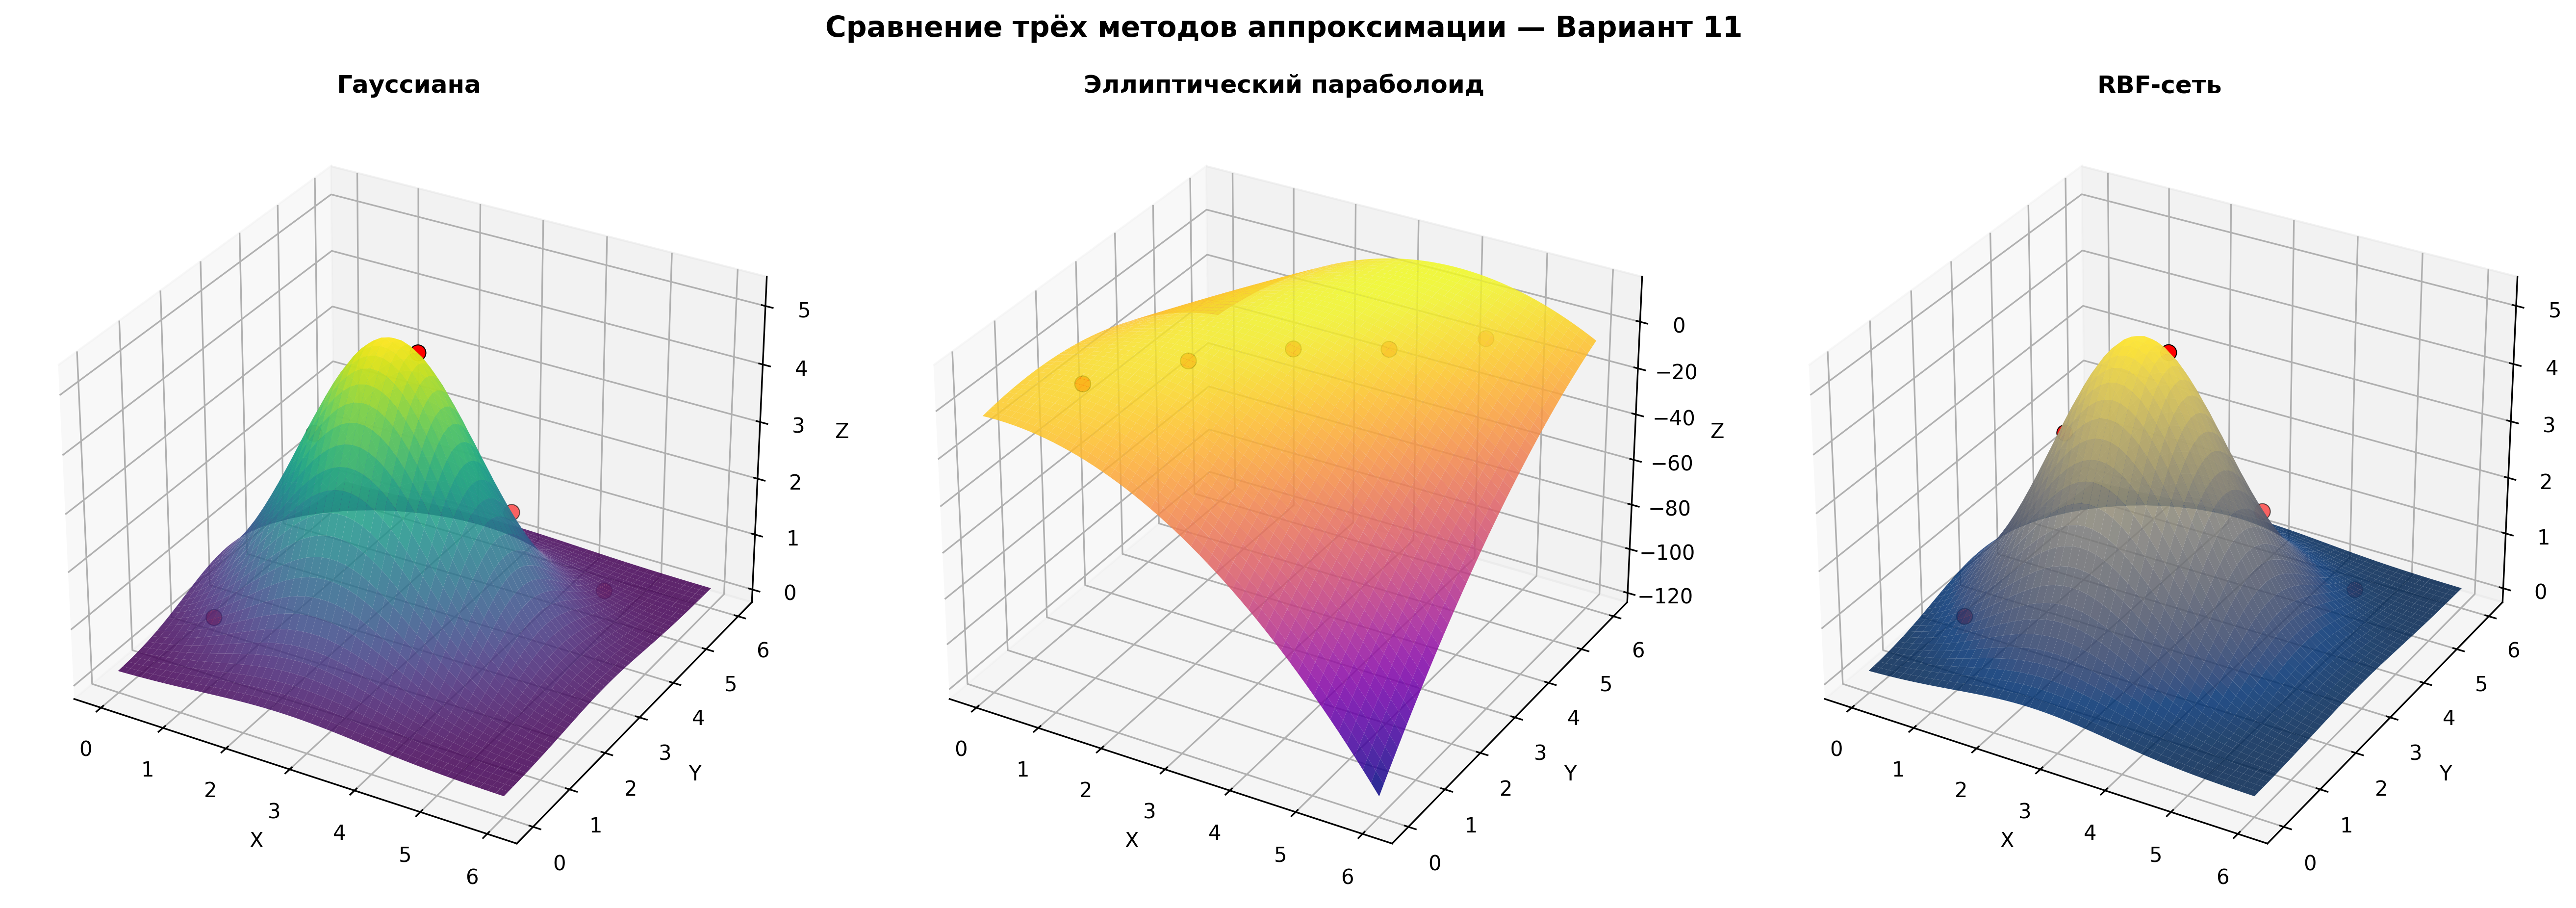
\includegraphics[width=\textwidth]{pic/all_models_3d.png}
    \caption{Сравнение 3D-поверхностей: Гауссиана (слева), Параболоид (центр), RBF-сеть (справа) --- Вариант 11}
    \label{fig:all_3d}
\end{figure}

\subsection{Анализ и общие выводы}

\begin{enumerate}
    \item \textbf{Гауссиана} ($\text{MSE} \approx 10^{-10}$) --- наилучшая модель. Данные варианта 11 порождены гауссовым распределением, поэтому модель восстанавливает зависимость с машинной точностью.

    \item \textbf{RBF-сеть} ($\text{MSE} \approx 10^{-6}$) --- отличная аппроксимация. Оба нейрона активны (веса $\approx 2.77$ и $2.28$), их центры близки и совместно формируют пик. Сумма двух гауссиан даёт большую гибкость, чем одна, однако MSE несколько выше из-за стохастической природы градиентного спуска и ограниченного числа эпох.

    \item \textbf{Параболоид} ($\text{MSE} = 0.0633$) --- приемлемая, но не отличная аппроксимация. MSE существенно ниже, чем в варианте 7 (0.714), что объясняется более симметричным расположением точек. Однако вершина $y_0 = 6.0$ вышла на границу, указывая на несоответствие формы параболоида гауссовым <<хвостам>>.

    \item \textbf{Константные модели} ($\text{MSE} \approx 3.0$) --- простейший baseline. Показывают, что данные имеют значительную вариацию ($\text{std}(z) \approx 1.72$), и осмысленная аппроксимация требует нелинейной модели.

    \item \textbf{Иерархия моделей по качеству:} Гауссиана $\succ$ RBF-сеть $\succ$ Параболоид $\succ$ Константа. Этот порядок объясняется соответствием функциональной формы модели истинной природе данных.
\end{enumerate}
